离散谱由连续谱之外的平方可积特征函数确定. 设三场满足命题 \ref{prop:evolution} 的正则性条件, 并取 $s_{22}$ 在 $D_+$ 中的有限个简单零点为 $\zeta_j$, 它们远离连续谱、$0$ 及共振原像; 共轭点为 $s_{11}$ 在 $D_-$ 中的零点.

\begin{proposition}[四点离散谱轨道]\label{prop:quartet}
若 $\zeta\in D_+$ 是 $s_{22}$ 的简单零点, 则
\begin{equation}\label{eq:quartet}
\left\{\zeta,\conj{\zeta},-\dfrac{q_0^2}{\zeta},-\dfrac{q_0^2}{\conj{\zeta}}\right\}
\end{equation}
构成完整四点轨道. 其中 $\zeta$ 与 $h(\conj{\zeta})$ 属于 $D_+$, 其余两点属于 $D_-$. 每个 $D_+$ 零点满足非零列相关关系
\begin{equation}\label{eq:norming-definition}
\phi_{+,2}(\zeta_j)=b_j\phi_{-,1}(\zeta_j),\qquad
c_j=\dfrac{b_j}{s_{22}'(\zeta_j)},\qquad
C_j=c_je^{2\ii\theta(\zeta_j)}.
\end{equation}
这里 $b_j,c_j$ 与 $x,t$ 无关, 撇号表示对单值化变量求导.
\end{proposition}
\begin{proof}
共轭与换叶各自改变 $\operatorname{Im}\lambda$ 的符号, 二者复合保留解析域. 由第五章的透射系数约化,
\[
s_{22}(\zeta)=0
\quad\Longrightarrow\quad
s_{11}(\conj{\zeta})=s_{11}(h(\zeta))=s_{22}(h(\conj{\zeta}))=0.
\]
$h'(z)=\dfrac{q_0^2}{z^2}\ne0$ 保持零点的简单性. 在连续谱之外, 四点互异. Wronskian 表达 \eqref{eq:wronskian} 表明 $\phi_{+,2}(\zeta)$ 与 $\phi_{-,1}(\zeta)$ 线性相关. 两列分别在正、负端指数衰减, 其共同张成的解在两端均平方可积. 非零解的列相关系数与 $x$ 无关; 命题 \ref{prop:evolution} 给出其 $t$ 不变性. 因而得到 \eqref{eq:norming-definition}.
\end{proof}

图 \ref{fig:discrete-spectrum} 给出一个轨道在单值化平面上的分布.
\begin{figure}[htbp]
\centering
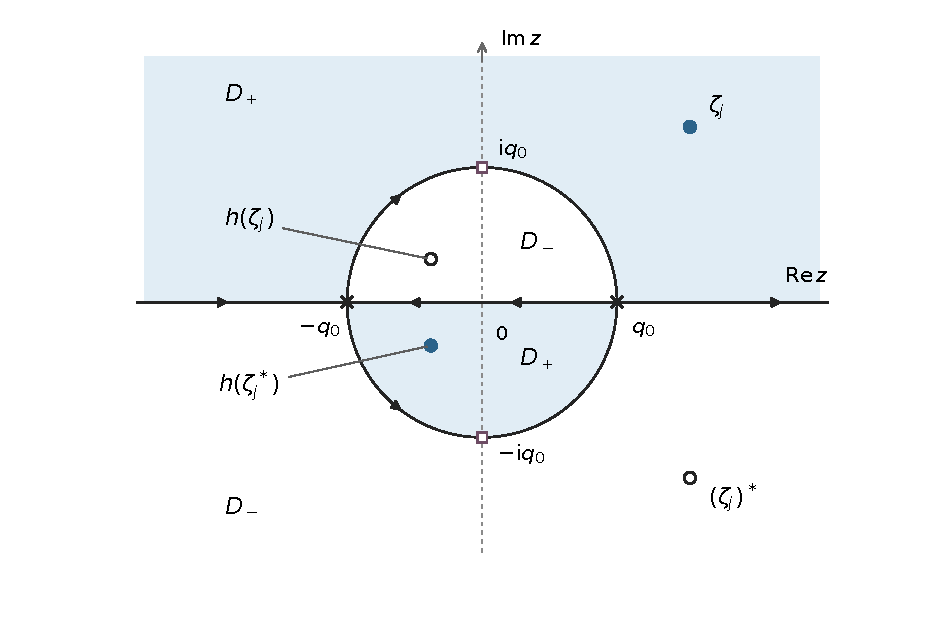
\includegraphics[width=0.78\textwidth]{figures/discrete-spectrum.pdf}
\caption{纯虚四点轨道, 图取 $q_0=1,a=2,W=\dfrac{3+\sqrt{5}}{2}$. 蓝点 $\zeta_1=\ii W$, $\zeta_2=h(\zeta_1^*)$ 为 $s_{22}$ 零点, 棕点为 $s_{11}$ 零点.}
\label{fig:discrete-spectrum}
\end{figure}

\begin{proposition}[简单零点的留数及常数约化]\label{prop:respair}
在式 \eqref{eq:norming-definition} 的条件下, 相应解析商满足
\begin{align}
\Res_{z=\zeta_j}\dfrac{\mu_{+,2}(z)}{s_{22}(z)}
&=C_j\mu_{-,1}(\zeta_j),\label{eq:resplus}\\
\Res_{z=\conj{\zeta_j}}\dfrac{\mu_{+,1}(z)}{s_{11}(z)}
&=-\conj{C_j}\mu_{-,2}(\conj{\zeta_j}).\label{eq:resminus}
\end{align}
若 $\widehat\zeta=h(\conj{\zeta})$ 为同一轨道的另一个 $D_+$ 点, 则
\begin{equation}\label{eq:cpair}
b_{\widehat\zeta}=-\conj{b_\zeta},\qquad
c_{\widehat\zeta}=-\dfrac{q_0^2}{(\conj{\zeta})^2}\conj{c_\zeta}.
\end{equation}
\end{proposition}
\begin{proof}
由 $\phi_{+,2}=b_j\phi_{-,1}$ 及 $\phi_1=\mu_1e^{\ii\theta}$、$\phi_2=\mu_2e^{-\ii\theta}$, 得到
\[
\mu_{+,2}(\zeta_j)=b_je^{2\ii\theta(\zeta_j)}\mu_{-,1}(\zeta_j).
\]
除以简单零点的导数便得 \eqref{eq:resplus}. 共轭约化逐列写为
\[
\phi_{\pm,1}(z)=\ii\sigma_2\conj{\phi_{\pm,2}(\conj{z})},\qquad
\phi_{\pm,2}(z)=-\ii\sigma_2\conj{\phi_{\pm,1}(\conj{z})}.
\]
所以在 $\conj{\zeta_j}$ 处,
\[
\phi_{+,1}=-\conj{b_j}\phi_{-,2},\qquad
s_{11}'(\conj{\zeta_j})=\conj{s_{22}'(\zeta_j)}.
\]
去除相位并除以导数, 得到负号留数 \eqref{eq:resminus}.

再在 $z=\conj{\zeta}$ 使用换叶关系. 它给出
\[
\phi_{+,2}(\widehat\zeta)
=\dfrac{\ii\conj{\zeta}}{q_0}\phi_{+,1}(\conj{\zeta})
=-\conj{b_\zeta}\dfrac{\ii\conj{\zeta}}{q_0}\phi_{-,2}(\conj{\zeta})
=-\conj{b_\zeta}\phi_{-,1}(\widehat\zeta).
\]
对恒等式 $s_{22}(h(z))=s_{11}(z)$ 求导, 有
\[
s_{22}'(\widehat\zeta)h'(\conj{\zeta})=\conj{s_{22}'(\zeta)},\qquad
h'(\conj{\zeta})=\dfrac{q_0^2}{(\conj{\zeta})^2}.
\]
这一步中的链式因子来自
$h(z)-\widehat\zeta=h'(\conj{\zeta})(z-\conj{\zeta})+O((z-\conj{\zeta})^2)$.
因此
\[
c_{\widehat\zeta}
=\dfrac{-\conj{b_\zeta}}{s_{22}'(\widehat\zeta)}
=-h'(\conj{\zeta})\conj{c_\zeta},
\]
即为 \eqref{eq:cpair}. 最后 $\theta(\widehat\zeta)=-\conj{\theta(\zeta)}$, 故这些常数关系同时保持留数的时空因子.
\end{proof}
